\documentclass[12pt]{article}
\usepackage{amsmath,amssymb,epsfig,bbm,ifthen,capt-of,calc}

%%%%%%%%%% Start TeXmacs macros
%\newcommand{\tmem}[1]{{\em #1\/}}
\newcommand{\tmfloatcontents}{}
\newlength{\tmfloatwidth}
\newcommand{\tmfloat}[5]{
  \renewcommand{\tmfloatcontents}{#4}
  \setlength{\tmfloatwidth}{\widthof{\tmfloatcontents}+1in}
  \ifthenelse{\equal{#2}{small}}
    {\ifthenelse{\lengthtest{\tmfloatwidth > \linewidth}}
      {\setlength{\tmfloatwidth}{\linewidth}}{}}
    {\setlength{\tmfloatwidth}{\linewidth}}  \begin{minipage}[#1]{\tmfloatwidth}
    \begin{center}
      \tmfloatcontents
      \captionof{#3}{#5}
    \end{center}
  \end{minipage}}
\newcommand{\tmop}[1]{\operatorname{#1}}
\newtheorem{theorem}{Theorem}
\newenvironment{proof}{
  \noindent\textbf{Proof}\ }{\hspace*{\fill}
  \begin{math}\Box\end{math}\medskip}
%%%%%%%%%% End TeXmacs macros

\newcommand{\tmem}[1]{\textit{#1}}
\newcommand{\tmfloatcontents}{}
\newcommand{\tmfloat}[5]{\newcommand{\tmfloatcontents}{#4}
{\setlength{{\tmfloatwidth}}{{\widthof{{\tmfloatcontents}}}+1in}} 

{\minipage{[#1]{\tmfloatwidth}
\begin{center}
  {\tmfloatcontents} {\captionof{#3}{#5}}
\end{center}}}}

\begin{document}
\title{Applications of Choice Theory: The Theory of
Demand}
\author{Michael Peters}
\date{\today}
\maketitle

\section{Introduction}

Preference Theory tells us that individuals who can express opinions about the
various alternatives available to them will act as if they are maximizing a
utility function. It is important to remember that this isn't meant to be a
description of what people actually do when they make decisions. Obviously
people don't consciously maximize anything when they make choices. Consumers
who never got the hang of finding $x$ in high school UNCLEAR--REFERENCE TO ALGEBRA??, nonetheless seem
perfectly capable of deciding how to spend their money. The basic presumption
in economics is that there is no way to know what people are actually thinking
when they make decisions.{\footnote{Not everyone agrees with this. For example
polling at elections is done under the assumption that respondents will
truthfully reveal who they want to vote for - they are often pretty close.
Psychologists often run experiments in which they simply ask people what they
would do if ... . Neuroeconomists believe that new brain scanning technology
will make it possible to observe preferences directly.}}

The fact that individuals' choices will look just like solutions to
maximization problems allows us to use methods and concepts from mathematics
to help describe behavior. The simple representations of behavior that
mathematics makes possible lead ultimately to the greatest contribution of
economics, the concept of {\tmem{equilibrium}} behavior. We will begin the
description of equilibrium behavior later on in this course.

To make use of the method that the utility theorem provides, we have to add
something to what we have so far. Suppose we are trying to figure out how
people will react to a price change. At the initial price, we can use the
theorem that we proved above to show that there is a utility function and that
the choices our consumer makes maximize this utility function subject to
whatever constraints she faces. The construction of this utility function
depends on the alternatives over which the consumer has to decide. There is
nothing in the theorem that says that the consumers preferences won't change
when the choice set does. Our consumer might believe that a higher price means
that the good she is buying has a higher quality than she initially thought.
After the price change she might `want' the good more than
before.{\footnote{My favourite example of this is Adobe Acrobat Software used
for making pdf files (like the file you are currently reading). There are many
free programs that will produce pdf files. Adobe's idea was that if they
offered an expensive software package to do the same thing, then people would
incorrectly believe that it was higher quality software. This strategy worked
brilliantly, at least among my colleagues who have jointly shelled out
thousands of dollars from their research grants to Adobe for free software -
thousands of dollars they could have paid to graduate students. DID CHRIS WRITE THIS?! HA! HA!}} Perhaps more
important, the price change might affect what other people do. Some goods are
more desirable when other people like and use them for
example.{\footnote{Telephones would be an obvious example. The fashion
industry seems to work on this principle. Advertize a brand name heavily (for
example, pay to have a celebrity use your product in a popular movie - ever
see I, Robot, or Italian Job?), then raise the product price to make it
exclusive. Suddenly everyone wants it and is willing to pay a lot for it. }}

To make use of the maximization approach, we need to make assumptions about
utility and how it changes when we change the environment. These assumptions
are called an economic {\tmem{model}}. Our economic model is what we use to
make the prediction. We will start with one of the oldest and perhaps simplest
economic models in the next section and I will explain what these extra
assumptions are and how to use the maximization approach to understand it "IT"' REFERS TO WHAT?? THE MODEL? THE ASSUMPTIONS?.

You might wonder about this "`THIS"' WHAT? APPROACH?. Doesn't this mean that economic predictions are
just elaborate assumptions about the way people behave? Why should I believe
these assumptions? If you are thinking this way, you are on the right track.
Economist spend an enormous amount of time and effort collecting and analysing
data - often with the view in mind of {\tmem{testing}} some economic model.
You'll be learning how to use models in this course, so we won't say much more
about testing, but we might find that our prediction is inconsistent with what
appears to be going on in the data we have collected. This may require that we
go back and revise the assumptions of our model to try to get things to work
out. So the assumptions evolve as more is learned about the way people behave.

Perhaps this leads you to a second, closely related question. If models are
just elaborate guesses about preferences designed to generate predictions, why
not just start right off with the predictions? For example, suppose we are
interested in the impact of an increase in price. It seems perfectly
reasonable to guess that if the price of good rises, then people will buy less
of it.{\footnote{This is called the Law of Demand. In October 1981, Senator
William Proxmire gave his Golden Fleece Award EXPLAIN THAT HE AWARDED THIS TO WHAT HE THOUGHT WAS THE GREATEST WASTE OF PUBLIC FUNDS to the National Science
Foundation for funding an empirical test of the Law of Demand. Pigeons in a
laboratory would receive food by pecking of a lever. Once the scientists had
trained the pigeons to peck on the lever to get food (the first ten years of
the project), they changed the rules so that the pigeons had to peck twice on
the lever to get food, instead of only once. The idea was that if the law of
demand holds, then pigeons should eat less when they have to peck twice than
they would if they only had to peck once. FINISH THE STORY!  IF I REMEMBER FROM CLASS, THEIR EXPERIMENT DID ACTUALLY 'PROVE' THE LAW OF DEMAD }} Why write down a maximization
model, find Lagrange multipliers, take derivatives, and all the other tedious
stuff? After all, we can always test our guess, and refine it if we are wrong.

There are basically two answers. Part of the answer is something universal
about using mathematics - it is something that everyone, no matter what their
field of study, knows. Formal mathematical models can in principal be
understood by everyone, not just specialists in economics. Apart from the
obvious connection with math and statistics, the modelling approach in
economics is similar to that used in some branches of computer science,
theoretical biology and zoology. In an odd way, formal modelling makes
economic theory more inclusive.

The real benefit (to all these fields) is that formal modelling helps make up
for the deficiencies in our own intuition. Our intuition is rarely wrong, but
it is almost always incomplete. It is also lazy. It wants to push every new
and challenging fact into an existing `intuitive' box, which makes us very
conservative intellectually. Careful mathematical analysis of well defined
models makes up for this. It helps us to see parts of the story that we might
not otherwise have noticed. It is often those insights gained through
painstaking mathematical analysis that lead to the most fundamental changes in
thinking. So if you spend hours thinking through the logic of one of the problems in
the problem set without actually getting the answer, don't despair. You are
often laying the groundwork for important leaps in your understanding that
will often transcend the particular problem you are working on.

At a more practical level, mathematical analysis will often reveal
implications of your model that your intuition would never have imagined.
These can often be critical. For example, it isn't hard to show that the law
of demand mentioned above need not be true. There is nothing in the nature of
preferences or the characteristics of markets that requires it to be true. If
our model doesn't tell us anything about demand curves, what use is it?
Rational behavior does impose restrictions on demand that are amenable to
econometric test. I will show you enough of the argument below for you to see
that the real implications of rational behavior in a market like environment
can not be understood using intuition, you need formal analysis.

Bear in mind as we go along, that the content of economics is not the
particular models we study, but the method of using models like this to
generate predictions, then modifying these until the predictions match the
information we have in our data.

\section{Consumer Theory}

A {\tmem{consumer}} is an individual who wants to buy some stuff. The `stuff'
will be a list of quantities of each of the goods that she wants. It is
natural to express this list as a {\tmem{vector}}, that is, an ordered list of
real numbers $x_1, x_2, \ldots, x_n$ where $x_1$ is the total number of units
of good 1 she wants, and so on. Refer to a generic {\tmem{bundle}} of goods as
$x \in \mathbbm{R}^n$, where this latter notation means that $x$ is an ordered
list consisting of exactly $n$ real numbers.

For the moment, let $\mathbbm{B}$ be the set of bundles that our consumer can
afford to buy. If we propose different alternatives in $\mathbbm{B}$ to our
consumer, she will be able to tell us which one she prefers. If these
preferences are transitive, then along with an appropriate continuity
assumption (see the previous chapter), there will be a utility function $u$
which converts bundles in $\mathbbm{R}^n$ into real numbers, and our consumer
will look just like she is maximizing $u$ when she chooses a bundle from $x$ THIS IS CONFUSING WITH THE $x$ BELOW. COULD WE INSTEAD REFER TO THE LIST AS $X$?

Now let $x$ and $y$ be a pair of alternatives in $\mathbbm{B}$. For the sake
of argument, suppose that $x \succeq y$ (which means that the consumer prefers
$x$ to $y$). Classical consumer theory makes two very strong assumptions. The
first is that the preferences of our consumer are independent of the
preferences and choices of all other consumers. The second is that preferences
are independent of the budget set that the consumer is offered. The first
assumption just means that we can think about one consumer in isolation. No
one really believes this is a good assumption, and we will begin to relax it
later on. It does make it much easier to explain the approach.

The second assumption can be stated more formally given the notation we have
developed. If the consumer prefers $x$ to $y$ when these are offered as
elements of $\mathbbm{B}$, then the consumer will still prefer $x$ to $y$ if
these are offered as choices from any other budget set $\mathbbm{B}'$.

What does this mean in words? Well as a good Canadian, you no doubt drink
foreign beer - Molson's (Coors USA), or Labatts (Interbrew, Belgium). Suppose
you would prefer a Molsons beer to a Labatt beer if you are given a
choice{\footnote{The presidents of Molson, Labatts and Big Rock Brewery
(Calgary) once went for a beer after attending a conference together. The
waiter asked the president of Labatt what he wanted to drink. He said proudly
``I'll have a Canadian''. ``Fine'' said the waiter. Then he asked the
president of Labatts, who said he would like a Labatt Blue. ``Fine'', said the
waiter, ``Good choice''. Then he asked the President of Big Rock. ``I'll have
a coke'', she said. ``Pardon?'' said the waiter. ``They aren't drinking beer
so I don't think I will either'', she replied.}}. If you suddenly won a lottery
that gave you  \$  1 million for life, would you still prefer a Molson to a
Labatt? Probably. You might not want a Molson or a Labatt, because you could
then afford to buy Champagne or something, but if you are given a choice
between those two only, you would probably still choose the Molson. That is
the nature of the second assumption.

Whatever you think of these two assumptions, let us accept them for the moment
and try to show how to draw out their implications.

\subsection{The Budget Set}

The set of consumption bundles that the consumer can afford is referred to as
the {\tmem{budget set}}. We can provide a mathematical characterization of
this set fairly easily. Lets assume that the consumer knows the prices of each
of the goods, and that these prices can be represented as a vector $p \in
\mathbbm{R}^n$, where $p$ is an ordered list $\{ p_1, \ldots p_n \}$. Lets
assume further that the consumer has a fixed amount of money $W$ to spend on
stuff. The set of consumption bundles that the consumer can afford to buy is
the set
\begin{equation}
  \left\{ x : x_i \geqslant 0 \forall i ; \sum_{i = 1}^n p_i x_i \leqslant W
  \right\} \label{budget}
\end{equation}
The brackets around the expression are used to describe the set. The notation
inside the bracket means the set of $x$ such that ($:$) each component of $x$
is at least as big as zero, and such that ($; )$ if you sum up the product of
the price and quantity across all components you end up with something less
than or equal to the amount of money you have to spend in the first place.
Hopefully you find the mathematical expression a lot more compact. However the
real benefit of using the math is yet to come.

It helps to mix formal arguments together which pictures like the ones you
saw in your first year course. To do this, imagine that there are only two
goods. Call them good $x$ and good $y$. The price of good $x$ will be $p_x$
and the price of $y$ will be $p_y$. The amount of money you spend buying good
$x$ is $p_x x$. The amount you spend on $y$ is $p_y y$. Total spending is $p_x
x + p_y y$ which can be no larger than what you have, $W$. That is exactly
what the math says in equation (\ref{budget}).

To help you think about this, lets also draw a picture.

\tmfloat{h}{small}{figure}{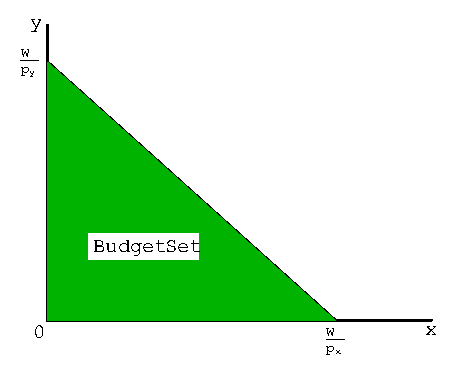
\epsfig{file=undergrad_demand_fig1.eps}
\label{udfig1} }{}

THE ALIGNMENT SEEMS TO BE OFF ON ALL THE FIGURES IN ALL THE NOTES.  TO MY EYE, THERE SHOULD BE A BIGGER SPACE BETWEEN THE LABEL AND THE TEXT BELOW IT.  AS WELL, THE COLON AFTER THE FIGURE IS UNNECESSARY, AND WASN'T IN THE OLD NOTES.  

In the picture above, our consumer has  \$ $W$ to spend on two different goods
called $x$ and $y$. If she spends her entire income on good $x$, she can
actually purchase $\frac{W}{p_x}$ units in all. This point is labelled on the
horizontal axis, and represents on feasible consumption bundle, i.e.,
$\frac{W}{p_x}$ units of good $x$ and no units of good $y$. By the same token,
she could spend all her money on good $y$, purchasing $\frac{W}{p_y}$ units of
good $y$, and no $x$. This point is labelled on the vertical axis as another
feasible consumption bundle.

Any combination of these two would also work. For example, half her income on
each good would yield a consumption bundle $( \frac{\frac{1}{2} W}{p_c},
\frac{\frac{1}{2} W}{p_y} )$. This bundle lies halfway along the line segment
that joins the points $( \frac{W}{p_x}, 0 )$ on the horizontal axis, and $( 0,
\frac{W}{p_y} )$ on the vertical axis.

She doesn't really have to spend all her money either. Since she doesn't have
any good $x$ or $y$ to sell, the set of feasible consumption bundles consists
of all the points in the triangle formed by the axis and the line segment
joining the point $( \frac{W}{p_x}, 0 )$ to the point $( 0, \frac{W}{p_y} )$.

The {\tmem{budget line}} is the upper right face of the triangle. The slope of
this line (rise over the run) is $- \frac{p_x}{p_y}$. The ratio of the price
of good $x$ to the price of good $y$ ($- 1$ times the slope of the budget
line) is called the {\tmem{relative price of good $x$}}.

\subsection{Using The Utility Theorem}

Implicitly, when we say that a bundle $( x, y )$ is at least as good as $( x',
y' )$, then we interpret this to mean that given the choice between the
bundles $\text{$( x, y )$}$ and $\text{$( x', y' )$}$ our consumer would
{\tmem{choose}} $\text{$( x, y )$}$. If that is true, then once we describe
the budget set, we must expect the consumer to choose a point in the budget
set that is at least as good as every other point in the budget set.  Our
`utility function' theorem says that as preferences are complete, transitive
and continuous, there will be a function $u$ such that a bundle $( x, y )$
will be at least as good as every other bundle in the budget set if and only
if $u ( x, y )$ is at least as large as $u ( x', y' )$ for every other bundle
$( x', y' )$ in the budget set. If we knew what this function $u$ was, then we
could find the bundle by solving the problem
\begin{equation}
  \max u ( x, y ) \label{objective}
\end{equation}
subject to the constraints
\begin{equation}
  p_x x + p_y y \leqslant W \label{budget-constraint}
\end{equation}
\begin{equation}
  x \geqslant 0 \label{x-positive}
\end{equation}
\begin{equation}
  y \geqslant 0 \label{y-positive}
\end{equation}
Now before we try to use the mathematical formulation, lets go back for a
moment to the characterization you learned in first year economics.

As we have assumed that the way our consumer ranks different bundles is
independent of the budget set that these bundles lie in, we can construct a
useful conceptual device. Take any bundle $( x, y )$. Form the set
\[ \{ \text{$( x', y' ) : \text{$( x, y ) \succeq \text{$( x', y' ) \tmop{and}
   \text{$( x', y' ) \succeq \text{$( x, y )$ \}}$}$}$}$} \]
In words, this is the set of all bundles $( x', y' )$ such that the consumer
is {\tmem{indifferent}} between $( x', y' )$ and $( x, y )$. This set is
referred to as an {\tmem{indifference curve}}. If the bundle $( x, y )$ is
preferred to the bundle $( x', y' )$, then every bundle in the indifference
curve associated with $( x, y )$ will be preferred to every bundle in the
indifference curve associated with $( x', y' )$. This follows by the
{\tmem{transitivity}} of preferences (remember that preferences are transitive
if $x \succeq y$ and $y \succeq z$ implies that $x \succeq z$). So the
consumer's choice problem outlined above is equivalent to choosing the highest
indifference curve that touches his or her budget set. DOESN'T THIS FIRST REQUIRE THE ASSUMPTION OF MONOTONICITY?? This gives the tangency
condition that you are familiar with, as in Figure \ref{tangency}.

\tmfloat{h}{small}{figure}{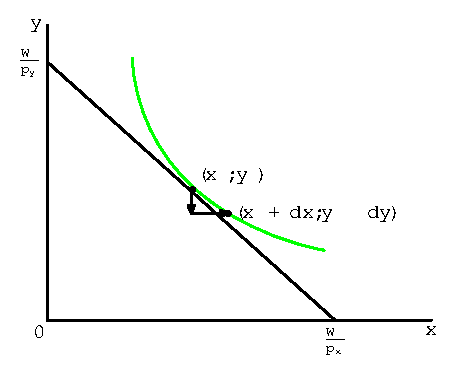
\epsfig{file=undergrad_demand_fig2.eps}}{\label{tangency}}

The two bundles $( x^{\ast}, y^{\ast} )$ and $( x^{\ast} + d x, y^{\ast} - d y
)$ both lie on the same indifference curve. The vertical distance $d y$ is the
amount of good $y$ that this consumer is willing to give up in order to get $d
x$ additional units of good $x$. When $d x$ is very small, the ratio of $d y$
to $d x$ is referred to as the {\tmem{marginal rate of substitution of $y$ for
$x$}}. Using your elementary calculus, notice that this marginal rate of
substitution is the same thing as the slope of the consumer's indifference
curve.

Now we can bring our utility theorem to bear. Assuming that the consumer's
preferences are complete, transitive and continuous, they must be represented
by some utility function, call it $u ( x, y )$. Then, the indifference curve
must be the set of solutions to the equation
\[ u ( x', y' ) = u ( x^{\ast}, y^{\ast} ) \]
Then we could calculate the slope of the indifference curve (that is, the
marginal rate of substitution) from the total differential
\[ u_x ( x, y ) d x + u_y ( x, y ) d y = 0 \]
or
\[ \frac{d y}{d x} = - \frac{u_x ( x, y )}{u_y ( x, y )} \]
where $u_x ( x, y )$ means the {\tmem{partial derivative}} of our utility
function $u$ with respect to $x$ evaluated at the point $( x, y )$.

Since the highest indifference curve touching the budget set is the one that
is just tangent to it, that means that the marginal rate of substitution of
$y$ for $x$ must be equal to the slope of the budget line $\frac{p_x}{p_y}$.

Now lets take the utility function that we know exists, and go back to the
purely mathematical formulation and maximize (\ref{objective}) subject to the
constraints (\ref{budget-constraint}) through (\ref{y-positive}). By the
Lagrangian theorem, there are three multipliers (one for each of the three
constraints) $\lambda_1, \lambda_2,$and $\lambda_3$ such the Lagrangian
function can be written as
\[ u ( x, y ) + \lambda_1 ( p_x x + p_y y - W ) - \lambda_2 x - \lambda_3 y \]
At the optimal solution to the problem, the following first order conditions
must hold
\begin{equation}
  u_x ( x, y ) + \lambda_1 p_x - \lambda_2 = 0 \label{x}
\end{equation}
\begin{equation}
  u_y ( x, y ) + \lambda_1 p_y - \lambda_3 = 0 \label{y}
\end{equation}
\begin{equation}
  p_x x + p_y y - W \leqslant 0 ; \lambda_1 \leqslant 0
\end{equation}
\begin{equation}
  - x \leqslant 0 ; \lambda_2 \leqslant 0
\end{equation}
\begin{equation}
  - y \leqslant 0 ; \lambda_3 \leqslant 0
\end{equation}
with the last three conditions holding with complementary slackness.

Suppose that we knew for some reason that the solution must involve positive
amounts of both $x$ and $y$ (you will see an example like this below). Then by
complementary slackness, the multipliers associated with both of these
variables would have to be zero. Then (\ref{x}) and (\ref{y}) would simplify
to
\[ u_x ( x, y ) = \lambda_1 p_x \]
and
\[ u_y ( x, y ) = \lambda_2 p_y \]
Dividing the first condition by the second gives exactly the same result that
we deduced from the picture
\[ \frac{u_x ( x, y )}{u_y ( x, y )} = \frac{p_x}{p_y} \]

\section{A Simple Example}

WHY DO YOU USE THIS EXAMPLE TWICE (HERE AND IN THE LAGRANGIAN NOTE)??

If we know more about the utility function, then the mathematical approach can
be quite helpful. For example, in the section of Lagrangian theory it was
assumed that the utility function had the form
\begin{equation}
  u ( x, y ) = x^{\alpha} y^{( 1 - \alpha )} \label{cobb-douglas}
\end{equation}
Then the first order conditions become
\begin{equation}
  \alpha x^{( \alpha - 1 )} y^{( 1 - \alpha )} + \lambda_1 p_x - \lambda_2 = 0
\end{equation}
\begin{equation}
  ( 1 - \alpha ) x^{\alpha} y^{- \alpha} + \lambda_1 p_y - \lambda_3 = 0
\end{equation}
\begin{equation}
  p_x x + p_y y - W \leqslant 0 ; \lambda_1 \leqslant 0 \label{cs3}
\end{equation}
\begin{equation}
  - x \leqslant 0 ; \lambda_2 \leqslant 0 \label{cs1}
\end{equation}
\begin{equation}
  - y \leqslant 0 ; \lambda_3 \leqslant 0 \label{cs2}
\end{equation}
where (\ref{cs3}), (\ref{cs1}) and (\ref{cs2}) hold with complementary
slackness. At first glance, this mess doesn't look particularly useful.
However, notice that if either $x$ or $y$ are zero, then utility is zero on
the right hand side of (\ref{cobb-douglas}). If the consumer has any income at
all, then she can do strictly better than this by purchasing any bundle where
both $x$ and $y$ are positive. As a consequence, we can be sure that at any
solution to the consumer's maximization problem, both $x$ and $y$ are
positive. Then by the complementary slackness conditions (\ref{cs1}) and
(\ref{cs2}), $\lambda_2$ and $\lambda_3$ must both be zero.

On the other hand, the solution will also require that the consumer use up
her whole budget since the right hand side of (\ref{cobb-douglas}) is strictly
increasing in both its arguments. Complementary slackness in (\ref{cs3})
unfortunately doesn't tell us that $\lambda_1$ is positive, it is possible,
but unlikely that both the constraint and its multiplier could be zero.

Lets continue. The logic of the Lagrange theorem is that the first order
conditions have to hold at a solution to the problem. Remember that the
converse is not true - a solution to the first order conditions may not give a
solution to the maximiztion problem. Now as long as both prices are strictly
positive, the fact that both $x$ and $y$ must also be strictly positive means
that if we find a solution to the maximization problem, then it must be that
this solution satisfies
\begin{equation}
  \alpha x^{( \alpha - 1 )} y^{( 1 - \alpha )} = - \lambda_1 p_x
  \label{simple-1}
\end{equation}
and
\begin{equation}
  ( 1 - \alpha ) x^{\alpha} y^{- \alpha} = - \lambda_1 p_y \label{simple-2}
\end{equation}
Now divide (\ref{simple-1}) by (\ref{simple-2}) (which means divide the left
hand side of (\ref{simple-1}) by the left hand side of (\ref{simple-2}) and
the same for the right hand sides). You will get
\begin{equation}
  \frac{\alpha}{1 - \alpha} \frac{y}{x} = \frac{p_x}{p_y}
\end{equation}
or $p_x x = p_y y \frac{\alpha}{1 - \alpha}$. Again, this last equation has to
be true at any solution to the maximization problem. Since it also has to be
true that $p_x x + p_y y = W$, then $p_y y \frac{\alpha}{1 - \alpha} + p_y y =
W$. This means that is has to be true that
\begin{equation}
  y = W ( 1 - \alpha ) / p_y \label{demand}
\end{equation}
Similarly $p_x = W \alpha / p_x$. These two equations are great because they
tell us the solution to the maximization problem for all different values of
$p_x$, $p_y$, and $W$. These last two equations are `demand curves', just like
the ones you saw in your first year economics course. You can easily see that
the `law of demand' holds for this utility function, an increase in price
lowers demand.

This simple example takes us a long way along the road to understanding what
it is that economists do differently from many other social scientists. We
started with some very plausible assertions about behavior - in particular,
given any pair of choices, consumers could always make one, and these choices
would be transitive. This showed us that we could `represent' these
preferences with a utility function. Using this utility function, we can
conclude that the consumers choice from any set of alternatives will be the
solution to a maximization problem.

By itself, this seems to say very little - if you give a consumer a set of
choices, she will make one. However, we now have the wherewithall to formulate
models - additional assumptions that we can add to hone our predicitions. We
added two of them. The first is basic to all the old fashioned consumer theory
- the way the consumer ranks any two bundles does not depend on the particular
budget set in which the alternatives are offered. The second assumption was
that the the utility function has a particular form as given by
(\ref{cobb-douglas}).

Putting these together we were able to apply some simple mathematics to
predict what the consumer would do in all the different budget sets that we
could imagine the consumer facing. This is the demand function (\ref{demand})
that we derived above. As promised above, the mathematics has delivered
{\tmem{all}} the implications of our model - the demand function shows that
there are a {\tmem{lot}} of implications, so it shouldn't be too hard for us
to check whether the model is right.{\footnote{It is both good and bad when a
model has lots of implications. It is good because it is easy to test. That
may make it a bad model as well if its predictions are obviously wrong. The
utility function in (\ref{cobb-douglas}) is like this. It predicts that the
consumer will consume positive amounts of every good - no sensible consumer
would pay for microsoft windows, or buy an SUV.UNCLEAR. THE JAB AT THE END OBSCURES THE MESSAGE. WHAT'S THE POINT?}} 

The theorem about the existence of the utility function allows us to unify our
approach (though not our model) to virtually all behavioral problems. We don't
even need to confine ourselves to human behavior. Animals make both behavioral
and genetic choices. Assuming that they are always able to make some choice
gives completeness, transitivity is arguably plausible, so we could represent
their choices as well as solutions to utility maximization problems. Genetics
involves choices made by biological systems in response to changes in
environmental conditions. Completeness and transitivity of these choices are
both compelling. Completeness is immediate. The idea that organisms evolve
seems to rule out the kind of cyclic choices implied by intransitivity (which
would require that one evolves then eventually reverts back again). So we
could try to model genetic behavior using the maximizing approach.{\footnote{I
can't resist suggesting one of my favourite arguments by Arthur Robson
(http://www.sfu.ca/~robson/wwgo.pdf). The formal title is ``Why we grow Large
and then grow old: Biology, Economics and Mortality'', the informal
title of his talk was ``Why we Die''. Yes, it is the solution to a
maximization problem.}}

The fact that we have a unified approach is nice, but not necessarily better.
After all we need to add a model (assumptions about utility, for example) that
could quite well be wrong. Fortunately, the econometricians have taught us how
to test our models and reject the ones that are wrong, so that we can refine
them. If you are taking econometrics MAYBE IT WAS JUST ME, BUT I DON'T THINK PEOPLE COMING OUT OF FIRST-YEAR KNOW WHAT ECONOMETRICS MEANS.  A SIMPLE EXPLANATION WOULD BE HELPFUL you might want to know how. If you take
logs of equation (\ref{demand}) you will get
\begin{equation}
  \log ( y ) = \log ( 1 - \alpha ) + \log ( W ) - \log ( p_y )
  \label{linear-equation}
\end{equation}
If you add an error term to this, you get a simple linear regression equation
in which the coefficient associated with the log of price is supposed to be 1.
That is very easy to test (and reject).

\section{How to Test Demand Theory}

If we make assumptions about the utility function, we can say a lot about how
consumers behave. As with the formuation given by (\ref{cobb-douglas}), these
strong predictions often won't be borne out in whatever data we have. For
example, an econometric test of (\ref{linear-equation}) will almost surely
fail. Then we can reject our model. However, we will most likely be rejecting
our assumption that the utility function has the form given in
(\ref{cobb-douglas}). What if we wanted to test the assertion that preferences
are independent of the budget set the consumer faces? To do that, we need to
find a prediction that will be true no matter what form the utility function
has, then find a situation where the consumer doesn't obey that prediction.

This creates a bit of a problem. Suppose our consumer simply doesn't care
what consumption bundle she gets. Then our model is consistent with any
pattern of behavior at all and we could never reject it. Neither would we find
such a model useful, because it doesn't really make any predictions. So a
useful and testable economic model will inevitably involve some assumptions
about the utility function.

Fortunately, if we simply add the assumption that consumers always prefer more
of a good to less of it, we get a prediction that is true no matter what other
properties the consumer's preferences have. It goes the following way -
suppose we observe at particular array of prices, a level of income, and the
choice the consumer makes under those circumstances. Then suppose it so
happens that at another time we observe a new array of prices, and a new level
of income that are such that the consumer could just afford to buy the
consumption bundle that she purchased in the first case. Of course, along this
new budget line we will get to observe another choice by the consumer. Along
this new budget line there will be some consumption bundles that would have
been inside (strictly) the budget set at the old prices and level of income.
If the consumer picks one of these then she is not acting as predicted by our
model, and we can reject our model.

Let me illustrate this in the simple case where there are only two goods. The
basic idea is depicted in Figure \ref{revealed}.

\tmfloat{h}{small}{figure}{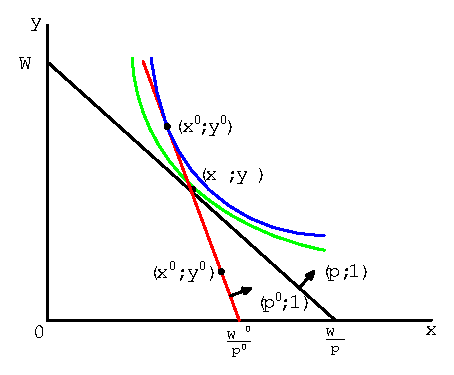
\epsfig{file=undergrad_demand_fig3.eps}}{\label{revealed}}

The point $( x^{\ast}, y^{\ast} )$ is the solution to the consumer's problem
at the inital set of prices. Here we simplify a bit by assuming that at the
initial situation, the price of good $x$ is $p$ while the price of good $y$ is
just $1$. The budget set for the consumer is the triangle formed by the axis
and the line between the points $( 0, W )$ and $( \frac{W}{p} )$.

Now we present the consumer with a new higher price for good $x$. The new
price is $p'$. At this new price, good $x$ is more expensive than it was
before, so our consumer could not afford to buy the bundle $( x^{\ast},
y^{\ast} )$ unless there is some change in her income. So lets suppose we can
give her just this income that she needs to buy the bundle $( x^{\ast},
y^{\ast} )$that she bought before the change in prices. This new income is
$W'$. This new income, along with the new price $p'$ gives her the blue budget
line, which by construction, just passes through the point $( x^{\ast},
y^{\ast} ) .$

This is all reasoning from your first year economics course. Along the new
budget line, the consumer should pick a point like $( x', y' )$. If she picks
a point like $( x^0, y^0 )$ instead, then she would be choosing a point that
she could have afforded to buy at the initial price $p$ before her income
changed.

What would be wrong with that? Well, remember, we are trying to figure out
whether our model is true. The model consists of three kinds of assumptions.
The first are our most basic axioms - completeness, transitivity and
continuity of preferences. The second is our assumption that preferences are
independent of the budget set that is presented to the consumer. The third is
the assumption that the consumer prefers more of each good to less.

Since $( x^0, y^0 )$ is inside the budget set when the price of $x$ is $p$ (we
leave out the additional qualifier ``and when income is $W$'' to make the
argument is little shorter IRONIC, NO?), then whatever the consumer's indifference curves
actually look like, there must be other bundles in the inital budget set that
are strictly preferred to $( x^0, y^0 )$. We have no idea what all these
bundles are, but suppose that one such bundle is $( x'', y'' )$ (which isn't
marked in the picture). Since the consumer chose $( x^{\ast}, y^{\ast} )$ from
that budget set, it must be that $( x^{\ast}, y^{\ast} )$ is at least as good
from the consumer's point of view as $( x'', y'' )$. Yet $( x'', y'' )$ is
strictly better than $( x^0, y^0 )$. Then by transitivity $( x^{\ast},
y^{\ast} )$ is strictly better for the consumer than $( x^0, y^0 ) .$ Then if
preferences are the same in every budget set, the consumer could do stricty
better in the new budget set at prices $p'$ by choosing $( x^{\ast}, y^{\ast}
)$. If our consumer chooses a bundle like $( x^0, y^0 )$ then there must be
something wrong with our story.

So if our model of the consumer is correct, we should observe that an
{\tmem{income compensated}} increase in the price of any commodity will result
in a fall in demand for that commodity. I will leave it to your econometrics
courses to tell you how the tests of consumer demand theory have worked out.

\section{Comparative Statics and The Envelope Theorem}

The idea that you need to understand to appreciate most modern economic
theory, is the idea that the consumer's choice depends on the constraint set
she faces. If we characterize the choice as the solution to a maximization
problem, then the consumers choice could be thought of as a {\tmem{function}}
of the parameters of the constraint set she faces. In general we refer to this
as a {\tmem{best reply}} function. In consumer theory the best reply function
is called a demand function. More generally the parameters that affect the
choice sets may not be prices. In game theory, the parameters that affect the
individual's choice behavior are the actions that she thinks others will take.

You have seen a best reply function already. When preferences are given by
(\ref{cobb-douglas}) then the amount of good $y$ the consumer will buy for
{\tmem{any}} pair of prices $( p_x, p_y )$ and {\tmem{any}} level of income
$W$ is given by (\ref{demand}). The demand for good $y$ is a function of its
price and the consumer's income.

It is actually pretty unusual to have the demand function in such a complete
form. To get such a thing, you actually need to be able to find a complete
solution to the first order conditions. That requires assumptions about
utility that are unlikely to pass any kind of empirical test. However, it is
often possible to use methods in mathematics to say useful things.

Lets go back to the case where preferences are represented by a function $u (
x, y )$ and assume that there is a demand function, say $D ( p_x, p_y, W )$
that tells us for each possible argument what quantity of good $x$ the
consumer will choose to buy. This function probably looks something like
(\ref{demand}), but we can't really say exactly what it is like. Lets make the
heroic assumption that this function looks like (\ref{demand}) in the sense
that it is differentiable, that is, $D ( p_x, p_y, W )$ has exactly three
partial deviatives, one for each of its arguments.

In particular, for preferences given by (\ref{cobb-douglas}), the demand
function for good $y$ is
\[ D ( p_x, p_y, W ) = \frac{( 1 - \alpha ) W}{p_y} \]
The three partial derivatives are given by
\[ \frac{\partial D ( p_x, p_y, W )}{\partial p_x} \equiv D_{p_x} ( p_x, p_y,
   W ) = 0 \]
\[ \frac{\partial D ( p_x, p_y, W )}{\partial p_y} \equiv D_{p_y} ( p_x, p_y,
   W ) = - ( 1 - \alpha ) W \left( \frac{1}{p_y} \right)^2 \]
\[ \frac{\partial D ( p_x, p_y, W )}{\partial W} \equiv D_W ( p_x, p_y, W ) =
   \frac{1 - \alpha}{p_y} \]
More generally, we can just refer to the partial derivatives as $D_{p_x}$,
$D_{p_y}$ and $D_W$ as long as you remember that these derivatives depend on
their arguments.

\subsection{Implicit Differentiation}

One method that will sometimes give you a lot of information about a best
reply function is implicit differentiation. To be honest, it doesn't really
work very well in demand theory, but I will explain it anyway. We will use
this method in our discussion of portfolio theory below.

Lets simplify things a bit and hold the price of good $y$ constant at 1 and
vary only the price $p$ of good $x$, and the level of income $W$. Lets suppose
as well that for some price $p$ and level of income $W$, the solution to the
consumer's maximization problem involves strictly positive amounts of both
goods $x$ and $y$. Then by the Lagrangian theorem, there must be a multiplier
$\lambda$ such that the first order conditions
\begin{equation}
  u_x ( x, y ) + \lambda p = 0 \label{foc21}
\end{equation}
\begin{equation}
  u_y ( x, y ) + \lambda = 0 \label{foc22}
\end{equation}
\begin{equation}
  p x + y = W \label{foc23}
\end{equation}
hold.

Then as we vary $p$ slightly, the values of $x$, $y$ and $\lambda$ will change
so that (\ref{foc21}) to (\ref{foc23}) continue to hold. Then by the chain
rule of calculus
\begin{equation}
  u_{x x} ( x, y ) \frac{d x}{d p} + u_{x y} ( x, y ) \frac{d y}{d p} +
  \lambda + p \frac{d \lambda}{d p} = 0
\end{equation}
\begin{equation}
  u_{y x} ( x, y ) \frac{d x}{d p} + u_{y y} ( x, y ) \frac{d y}{d p} +
  \frac{d \lambda}{d p} = 0
\end{equation}
\begin{equation}
  x + p \frac{d x}{d p} + \frac{d y}{d p} = 0
\end{equation}
In this notation, the terms like $u_{x x} ( x, y )$ are second derivatives.
For example, when preferences are given by (\ref{cobb-douglas}), $u_{x x} ( x,
y ) = \alpha ( \alpha - 1 ) x^{\alpha - 2} y^{1 - \alpha}$. The terms like
$\frac{d x}{d p}$ are the derivatives of the implicit functions that satisfy
the first order conditions (\ref{foc21}) to (\ref{foc23}) as $p$ changes a
little.

We are interested in trying to figure out properties of $\frac{d x}{d p}$. In
principle, we could use these last three equations to learn about it. There
are three equations and three unknowns. They are non-linear, so there is no
guarantee they will have a solution, but they probably will. The complication
is that this solution is complicated and won't actually say much. For what it
is worth, pure brute force gives the following
\begin{equation}
  \frac{d x}{d p} = \frac{( u_{x y} - p u_{y y} ) x - \lambda}{u_{x x} - 2 p
  u_{x y} - p^2 u_{y y}} \label{cs}
\end{equation}
This is pretty bleak, because there is too much in the expression that we
don't know. The sign of the expression could be either positive or negative
depending on the sizes of the cross derivatives. Then there is the mysterious
multiplier term $\lambda$.

The one advantage this approach does have is that it will often tell you what
you need to {\tmem{assume}} in order to get the result that you want. Since
the irritating terms are the cross derivatives, suppose that we make the
utility function {\tmem{separable}}. For example, it might have the form $u (
x, y ) = v ( x ) + w ( y )$ where $v$ and $w$ are concave functions (which
means that their derivatives get smaller as their arguments get larger). Then
$u_{x y} = u_{y x} = 0$ and (\ref{cs}) reduces to
\begin{equation}
  \frac{d x}{d p} = \frac{- p w_{y y} x - \lambda}{v_{x x} - p^2 w_{y y}}
\end{equation}
This still not enough. If we assume that the function $u$ and $v$ are both
concave then their second derivatives can't be negative CONCAVE MEANS BOTH PRECISELY THAT BOTH SECOND DERIVATIVES ARE NEGATIVE, RIGHT?!?. The multiplier is
less than or equal to zero by the complementary slackness conditions, so the
numerator is non-negative. The denominator can be either positive or negative
depending on the magnitudes of the second derivatives.

This leads us to the second most famous special functional form in economics.
If we assume that $w ( y ) = y$, we get something called a
{\tmem{quasi-linear}} utility function. Then $w_{y y} = 0$ and we know that
the demand function is at least downward sloping. Quasi linear utility
functions are widely used in the theory of mechanism design and auctions.

\subsection{Graphical Methods}

The arguments above are a bit obscure. Graphical methods will often provide
some more insight. The methods in the previous section are also {\tmem{local}}
methods, since they assume that all the changes that are occuring are small.
Graphical analysis won't really give you a full solution to the problem you
are trying to solve, you will ultimately need to return to the math for a full
solution. Yet graphical analysis will often point in the right direction.

If you simply want to understand why the demand function doesn't slope
downward, a graphical trick will show you. Go back to Figure \ref{revealed}
where the consumer was faced with an increase in the price of good $x$, but
was given enough income to allow her to afford her initial consumption bundle.
We concluded that this combination of changes in her budget set would induce
her to lower her demand for good $x$. We can decompose these changes into
their constitutent parts - an increase in price, followed by an increase in
income. The two changes together appear in Figure \ref{slutsky}.

\tmfloat{h}{small}{figure}{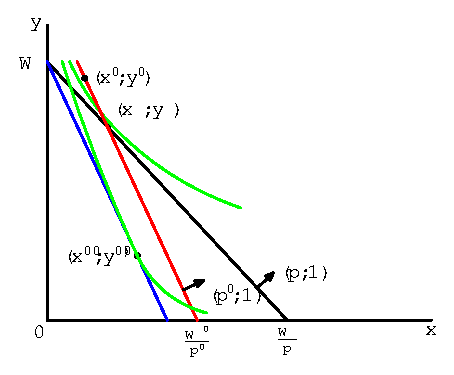
\epsfig{file=undergrad_demand_fig4.eps}}{\label{slutsky}}

The picture shows a problem similar to the one in Figure \ref{revealed}. The
initial price for good $x$ is $p$. At the price and her initial income, the
consumer selects the bundle $( x^{\ast}, y^{\ast} )$. As we saw before, if we
raise the price of good $x$ to $p'$ but give the consumer enough extra income
that she could just purchase the original bundle $( x^{\ast}, y^{\ast} )$,
then she must respond by puchasing more good $y$. In other words, her
compensated demand for good $x$ must fall. For example, she might choose the
new bundle $( x', y' )$ as in the Figure.

If we want to know how the impact of the price increase by itself will
influence her demand, we need to take away the extra income we gave her so
that she could afford her intial bundle. In the picture we do this by shifting
the budget line downward (toward the origin) from the red line to the blue
line. Since we are holding both prices constant as we take away this income,
the slope of the budget line doesn't change as we shift it in. (Make sure you
understand why the blue line goes through the point $( 0, W )$.

As the picture is drawn, our consumer chooses the bundle $( x'', y'' )$. The
remarkable thing about this bundle is that it actually involves more good $x$
than there is in the initial bundle $( x^{\ast}, y^{\ast}$). An increase in
the price of good $x$ has actually caused an increase in demand for good $x$.
The diagram illustrates why. As our consumers income rises (shifting the
budget line up from the blue line to the red line, her demand for good $x$
actually falls. Goods that have this property are called {\tmem{inferior
goods}} as you  may recall from your first year course.

\subsection{The Envelope Theorem}

There is one special theorem associated with the Lagrangian that is sometimes
quite useful. Suppose that we are trying to solve the problem
\begin{equation}
  \max_x u ( x )
\end{equation}
subject to
\begin{equation}
  G_1 ( x, y ) \leqslant 0
\end{equation}
\[ \vdots \]
\begin{equation}
  G_m ( x, y ) \leqslant 0
\end{equation}
where $x \in \mathbbm{R}^n$, $m \geqslant 1$, and $y$ is some parameter that
affects our constraints, for example, the price of one of the goods, or the
consumer's income. If we could find a solution to this problem, the we could
call the {\tmem{value}} of the solution $V ( y )$. This value is a function of
the parameter $y$. If $y$ were a price, for instance, then the maximum value
of utility would be a decreasing function of price. Suppose we are interested
in finding out how a change in $y$ will change this maximum value - i.e., we
want to know something about $\frac{d V ( y )}{d y}$.

One way to do this to use implicit differentiation as we did above. The vector
$x^{\ast}$ that solves the problem is an implicit function of $y$. Imagine
that $x^{\ast} [ y ]$ is the function that gives us the solution to the
problem. For example, in the consumer's problem, if we think of $y$ as the
price of good $x$, then $x^{\ast} [ y ]$ is the {\tmem{bundle}} that provides
the maximum utility. Whatever the actual interpretation, it should be clear
that $V [ y ] = u [ x^{\ast} [ y ] ]$. We could then compute the impact of a
change in $y$ by finding all the partial derivatives of $u$ with respect to
each of the $x$'s evaluated at the intial optimal solution, multiplying each
of these by the total derivative of the correponding solution with respect to
a change in $y$, then summing everything up. In math
\[ \frac{d V ( y )}{d y} = \sum_{i = 1}^n \frac{\partial u ( x^{\ast} [ y ]
   )}{\partial x_i} \frac{d x^{\ast}_i [ y ]}{d y} \]
This would require not only that we take a lot of partial derivatives, but
also that we compute function $x^{\ast} [ y ]$ and find its total derivatives
- a daunting amount of work.

Fortunately, there is a very nice way around this. Recall that the Lagrangian
function associated with this maximization problem is
\[ L ( x, \lambda, y ) = u ( x ) + \sum_{j = 1}^m \lambda_j G_j ( x, y ) \]
Then the envelope theorem says that

\begin{theorem}
  \begin{equation}
    \left. \frac{d V ( y )}{d y} = \frac{d L ( x, \lambda, y )}{d y}
    \right|_{x = x^{\ast} ; \lambda = \lambda^{\ast}}
  \end{equation}
\end{theorem}

The notation at the end means that we evaluate the total derivative of the
Lagrangian function at the solution to the problem. This says that if we can
just find the solution to the problem (both the optimal $x$'s and the
multipliers $\lambda$ that satisfy the first order conditions), then we can
find the derivative we want by evaluating a simple total derivative.

I am going to show you why this is true, but first I'll show you how it works.
Our consumer solves the problem
\[ \max u ( x, y ) \]

THE NOTATION IS INCONSISTENT AND CONFUSING BECAUSE y WAS THE PARAMETER ABOVE AND NOW IT'S A CHOICE VARIABLE

subject to
\[ p x + y - W \leqslant 0 \]

\[ - x \leqslant 0 \]
\[ - y \leqslant 0 \]
The Lagrangian is
\[ u ( x, y ) + \lambda_1 ( p x + y - W ) - \lambda_2 x - \lambda_3 y \]
Suppose I want to find out the impact of an increase in wealth on the
consumer's optimal utility starting from an initial price $p_0$ and wealth
level $W_0$. The Envelope theorem says that we first need to solve the
consumer's problem and find the utility maximizing demand, call them $x^0$ and
$y^0$, as well as the multipliers that satisfy the first order conditions at
the optimal solution, $\lambda^0_1$, $\lambda^0_2$, and $\lambda^0_3$. The
Lagrangian is generally a complicated function of $W$ because all the
multipliers and the optimal $x$ and $y$ are changing with $W$. Nonetheless the
derivative of this optimal value is simply
\[ \frac{d L ( x, y, \lambda_1, \lambda_2, \lambda_3 )}{d W} = - \lambda \]
The significance of the $d L$ instead of $\partial L$ is that we don't have to
worry about all the implicit functions.

Here is the proof of the envelope theorem:

\begin{proof}
  First observe that
  \[ V [ y ] = L ( x^{\ast}, \lambda^{\ast}, y ) \]
  \begin{equation}
    = u ( x^{\ast} ) + \sum_{j = 1}^m \lambda^{\ast} G ( x^{\ast}, y )
  \end{equation}
  It might seem that this would be false because of the sum that we add to $u
  ( x^{\ast} )$. However, by the complementary slackness conditions, the
  product of the multiplier and the constraint will always be zero at the
  solution to the first order conditions. So the sum is exactly zero.
  
  As long as we think of $x^{\ast}$ and $\lambda^{\ast}$ as implicit functions
  of $y$, then this is an identity, so we find the derivative using the chain
  rule.
  \[ \frac{d V ( y )}{d y} = \sum_{i = 1}^n \frac{\partial u ( x^{\ast}
     )}{\partial x_i} \frac{d x^{\ast}_i}{d y} + \sum_{j = 1}^m \left[ \frac{d
     \lambda_j^{\ast}}{d y} G_j ( x^{\ast}, y ) + \lambda^{\ast}_j \sum_{i =
     1}^n \frac{\partial G_j ( x^{\ast}, y )}{\partial x_i} \frac{d
     x^{\ast}_i}{d y} + \lambda^{\ast}_j \frac{d G_j ( x^{\ast}, y )}{d y}
     \right] \]
  First consider the terms $\frac{d \lambda_j^{\ast}}{d y} G_j ( x^{\ast}, y
  )$. By complementary slackness, either $G_j ( x^{\ast}, y )$ is zero, or
  $\lambda^{\ast}_j$ is zero, or both are zero. In the first case, and the
  last case, we can forget about the term $\frac{d \lambda_j^{\ast}}{d y} G_j
  ( x^{\ast}, y )$ because it will be zero. What happens when $G_j ( x^{\ast},
  y ) < 0$? In that event changing $y$, say by $d y$, will not change anything
  about the solution very much and we can rely on continuity to ensure that
  $G_j ( x^{\ast} [ y + d y ], y + d y )$ is still negative. If that is the
  case, then again using complementary slackness, it must be that
  $\lambda^{\ast}_j [ y + d y ] = 0$, which means that $\frac{d
  \lambda^{\ast}_j}{d y}$=0.
  
  Using this, we can rewrite the derivative as follows
  \[ \frac{d V ( y )}{d y} = \sum_{i = 1}^n \left( \frac{\partial u ( x^{\ast}
     )}{\partial x_i} + \sum_{j = 1}^m \lambda^{\ast}_j \frac{\partial G_j (
     x^{\ast}, y )}{\partial x_i} \right) \frac{d x^{\ast}_i}{d y} + \sum_{j =
     1}^m \lambda^{\ast}_j \frac{d G_j ( x^{\ast}, y )}{d y} \]
  Now notice that the terms in the first sum over $i$ are all derivatives of
  the Lagrangian with respect to some $x_i $evaluated at the optimal solution.
  Of course the optimal solution has the property that ther derivatives of the
  Lagrangian with respect to the $x_i$ are all equal to zero. Consequently the
  derivative reduces to
  \[ \frac{d V ( y )}{d y} = \sum_{j = 1}^m \lambda^{\ast}_j \frac{d G_j (
     x^{\ast}, y )}{d y} \]
  which is just the simple derivative of the Lagrangian with respect to the
  parameter $y$.
  
  
\end{proof}

\end{document}
